\chapter{Экспериментальный раздел}
\label{cha:research}
    В данном разделе будут проведены эксперименты для проведения 
    сравнительного анализа алгоритмов по затрачиваемому процессорному 
    времени в зависимости от размера матрицы.[\ref{bib:2}]
    \section{Сравнительный анализ на основе замеров времени работы алгоритмов}
        В рамках данного проекта были проведёны следующие эксперименты:

        1) сравнение времени работы алгоритмов при нечетном размере массива(график \ref{graph:test:1});
        2) сравнение времени работы алгоритмов при четном размере массива(график \ref{graph:test:2}).

        
        Тестирование проводилось на компьютере с процессором
        Intel(R) Core(TM) i5-8265U CPU @ 1.60GHz 1.80 GHz под управлением Windows 11 с 8 Гб оперативной памяти.\\

        \begin{figure}[h!]
            \centering
            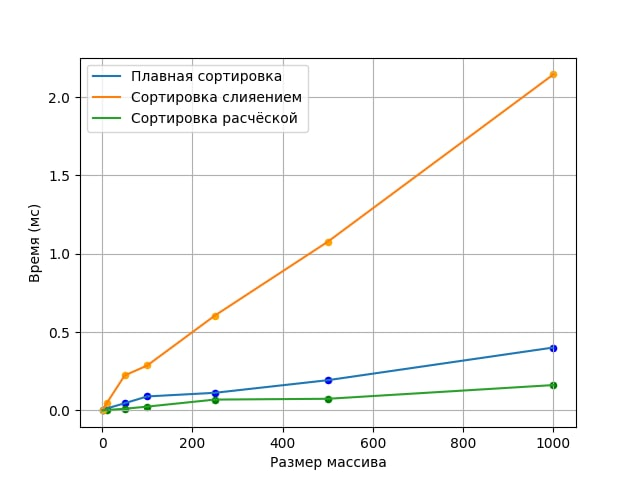
\includegraphics[scale=0.9]{graph_1.png}
            \caption{Зависимость времени работы алгоритмов от размера матрицы, если он нечетный}
            \label{graph:test:1}
        \end{figure}
        \newpage
        \begin{figure}[h!]
            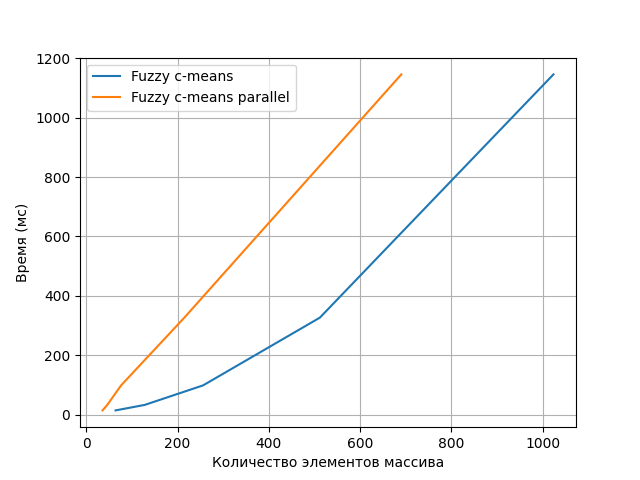
\includegraphics[scale=0.9]{graph_2.png}
            \caption{Зависимость времени работы алгоритмов от размера матрицы, если он четный}
            \label{graph:test:2}
        \end{figure}
        \newpage

    \subsubsection*{Оптимизация в компиляторе}
    \par Аппелируя к графикам выше, можно сделать вывод, что алгоритм с оптимизацией работает быстрее, но важно помнить, что компилятор делает некоторые из этих оптимизаций самостоятельно.
    \par Например, замена умножения на 2 на побитовый влево заменяется компилятором GCC на сложение, а PowerPC делает замену как раз таки на побитовый свдиг.[\ref{bib:5}] 

    \section{Вывод}
        \par В ходе экспериментов по замеру времени работы было установлено, что независимо от четного или нечетного размера матрицы алгоритм Винограда с оптимизацией работает быстрее, чем алгоритм Винограда без нее и алгоритм классического умножения матриц.



\newpage